%% Change "letterpaper" in the following line to "a4paper" if you must.

\documentclass[10pt,a4paper]{article}
\usepackage{cogsci}
\usepackage{pslatex}
\usepackage{apacite}


%\usepackage{geometry}
\usepackage{natbib}
\bibpunct[:]{(}{)}{,}{a}{}{;}

\usepackage{amsmath}
\usepackage{amsfonts}
\usepackage{amsthm}
\usepackage{amssymb}
\usepackage{mathrsfs}
\usepackage{nicefrac}
%\usepackage{stmaryrd}
%\usepackage{multicol}
\usepackage{graphicx}
\usepackage{caption}
\usepackage{subcaption}
\usepackage{color}
\usepackage{booktabs}

\usepackage{blkarray}
\usepackage{xspace}


\definecolor{Red}{RGB}{178,34,34}
\newcommand{\mf}[1]{\textcolor{Red}{[MF: #1]}} 
\newcommand{\tb}[1]{\textcolor[rgb]{.8,.33,.0}{[TB: #1]}}% prints in orange
\newcommand{\citeposs}[2][]{\citeauthor{#2}'s (\citeyear[#1]{#2})}
\newcommand{\tuple}[1]{\ensuremath{\left\langle #1 \right\rangle}} 


%%% MF's commands
\newcommand{\set}[1]{\left\{#1\right\}}
\newcommand{\card}[1]{\left \lvert \, #1 \, \right\rvert}
\newcommand{\abs}[1]{\lvert #1 \rvert}
\newcommand{\States}{\ensuremath{S}\xspace}		% Set of States
\newcommand{\state}{\ensuremath{s}\xspace}		% single states
\newcommand{\mystate}[1]{\ensuremath{\state_{\text{#1}}}\xspace} %meaningful states
\newcommand{\Messgs}{\ensuremath{M}\xspace}		% Set of Messages
\newcommand{\messg}{\ensuremath{m}\xspace}		% single messages
\newcommand{\mymessg}[1]{\ensuremath{\messg_{\text{#1}}}\xspace} %meaningful messages
\newcommand{\ssome}{\mystate{\ensuremath{\exists\neg\forall}}}
\newcommand{\sall}{\mystate{\ensuremath{\forall}}}
\newcommand{\msome}{\mymessg{some}}
\newcommand{\mall}{\mymessg{all}}
\newcommand{\asome}{\myact{\ensuremath{\exists\neg\forall}}}
\newcommand{\aall}{\myact{\ensuremath{\forall}}}
\definecolor{mygray}{cmyk}{0.35,0.35,0.35,0.35}
\newcommand{\mygray}[1]{{\textcolor{mygray}{#1}}}


%\citeA{bibkeyword} cites only year

\title{Systematic transmission perturbations in the cultural evolution of language}
 
\author{{\large \bf Name Surname (mail@mail.com)} \\
  Department, street \& number \\
  city, ZIP country
  \AND {\large \bf Name Surname (mail@mail.com)} \\
  Department, street \& number \\
  city, ZIP country}


\begin{document}
\maketitle

\begin{abstract}
Over time, languages favors linguistic features that can be passed on with high fidelity from one language user to the next. The outcomes of this process are often argued to involve cognitive biases that influence a learner's inductive task. Such learning biases thereby serve as central devices to understand and predict linguistic structure. We complement this view by showing how such effects can also arise without assuming any biases but simply as an epiphenomenon of systematic disturbances stemming from environmental factors. To this end, we investigate the effects of iterated learning under noisy perception in three case studies on (i) vagueness, (ii) meaning deflation, and (iii) a lack of upper-bounds in weak scalar alternatives. We argue these technical results to underpin the importance of, either cognitive or extraneous, transmission perturbations in the cultural evolution of language and bring attention to the often overlooked possibility that channel noise can mimic effects of inductive biases.

\textbf{Keywords:} 
noise; cognitive biases; iterated learning; cultural evolution;  
\end{abstract}
\section{Introduction}
Language is shaped by its use and transmission across generations. Linguistic properties therefore need not necessarily arise and stabilize solely due to functional pressure but may also be influenced and selected for by a pressure for learnability. The effects that such iterated learning has on language can be viewed as arising from a combination of general learning mechanisms and inductive cognitive biases (e.g. \citealt{griffiths+kalish:2007,kirby+etal:2014,tamariz+kirby:2016}). Proposals of biases that shape language acquisition abound. Some prominent examples are mutual exclusivity \citep{merriman+bowman:1989,clark:2009}, simplicity \citep{kirby+etal:2015}, regularization \citep{hudson+etal:2005}, and generalization \citep{smith:2011,oconnor:2015}.\footnote{Depending on their formulation and the domain(s) they are proposed to apply to, biases may also interact. For instance, a domain-independent bias for simplicity may entail regularization but stand in conflict with mutual exclusivity.} In the following we show how environmental factors can produce evolutionary outcomes that look as if such cognitive learning biases are present even if they are not.

We present three case studies that show how transmission perturbations can lead to well-known linguistic phenomena: vagueness, meaning deflation, and a lack of upper-bounds in weak scalar expressions. These results are not meant to suggest noisy perception to be the sole or main determinant of these phenomena. Instead, this investigation's main contribution is conceptual and seeks to underline the pivotal role of systematic transmission perturbations of linguistic knowledge in language change while showing that such perturbations may stem from other sources, e.g., from learners' noisy perception.


\section{Iterated learning under noisy perception}
We model the transmission of linguistic knowledge as process of iterated learning (for recent overviews see \citealt{kirby+etal:2014, tamariz+kirby:2016}). That is, as a repeated transfer of knowledge and behavior, such a language and its use, from one agent to another. 

In the simplest case one may think of this process as involving a chain of parents and children. At the chain's top a parent produces linguistic data. This data is witnessed by the next agent in the chain, a child, who in turn acquires a language and behavior based on it. The child, now turned a proficient adult language user, then goes on to produce data for another child to learn from and so on. The learner's task is therefore to infer covert linguistic information, such as a language's grammar or when {\em red} holds true of an object, from observable language use. Importantly, there are multiple ways in which this process can induce change in a language. For instance, learning data may be sparse, speaker may make mistakes in production, or it could be that data incorrectly perceived by the learner. The fidelity by which a language or feature is transmitted against such perturbations therefore plays an important role in its emergence and stability across generations.

If linguistic behavior is kept constant across agents then the learner's task reduces to inferring a language $L \in \mathcal{L}$. A more general approach, used in our third case study, is to allow for variation in an agents production algorithm as well \citep{brochhagen+etal:2016:CogSci}. In these cases the learner's task is to perform a joint inference over types of linguistic behavior and lexical meaning. We call such a combination a type, $t \in T$. 

More precisely, we follow \citet{griffiths+kalish:2007} in modeling language acquisition as a form of (iterated) Bayesian learning \citep{griffiths+kalish:2007}. Learning is hereby captured as a combination of the likelihood of a type generating the data witnessed by the learner with prior inductive biases, $P \in \Delta(T)$. This prior can be understood as a condensed codification of learning preferences. For example, learners may have a preference for simpler languages over ones with a more complex grammar, larger or more marked inventories, or cognitively taxing components (c.f. \citealt{feldman:2000,chater+vitanyi:2003, kirby+etal:2015}). Crucially, even weak biases can magnify and have striking effects on an evolving linguistic system. Experimental and mathematical investigations in iterated learning have therefore been taken to suggest that the linguistic structure evinced by the outcome of this process reflect learners inductive biases \citep{kirby+etal:2007,kirby+etal:2014}. 

The set of possible data a learner may be exposed to is represented by a set $D$. This set is made up of $k$-length sequences of the form $\tuple{\tuple{s_i,m_j}, ..., \tuple{s_k,m_l}}$, where $s \in S$ is the observation of meaning $s$ accompanied with an utterance $m \in M$. The parameter $k$ therefore controls how much information learners have at their disposition to discern languages from one another. Generally, low $k$ means that more languages will be compatible with the data, lowering the likelihood of a language being passed on faithfully. Conversely, inferring the language that generated the data, i.e., adopting the language used by a teacher, has a higher likelihood for larger sequences. 


The likelihood $P(d|t_j)$ of datum $d$ being produced by type $t_j$ is given by a parent $j$'s linguistic behavior in combination with the language it uses. Letting $P_{PA_j}(\cdot)$ and $L_j$ stand type $j$'s production algorithm and language:

\begin{align*}
  P(d = \tuple{\tuple{s_1,m_1},\dots , \tuple{s_k,m_k}} \mid t_j) = \prod_{i = 1}^k P_{PA_j}(m_i
  \mid s_i; L_{j})\,.
\end{align*}



These components can be put together in a transmission matrix $Q$, where $Q_{ij}$ is the probability that a learner acquires language $i$ when learning from a user of language $j$

\begin{flalign*}
  Q_{ji} \propto \sum_{d \in D} P(d \mid t_j) F(t_i \mid d)\,.
\end{flalign*}

where $F(t_i \mid d)$ is the parametrized acquisition probability of $t_i$ given datum $d$, obtained from the likelihood and prior:

\begin{flalign*}
  & F(t_i \mid d) \propto [P(t_i) P(d \mid t_i)]^l\,.
\end{flalign*}

where $l$ is a posterior parameter \tb{explain and then go over to noise}.


\paragraph{Noisy transmission}
We denote the probability that the teacher (learner) observes state $s_t$ ($s_l$) when the actual state is $s_a$ as $P_N(s_t \mid s_a)$ ($P_N(s_l \mid s_a)$). The probability that $s_a$ is the actual state when the learner observes $s_l$ is therefore:

\begin{align*}
  P_N(s_a \mid s_l) \propto P(s_a) \ P_N(s_l \mid s_a)\,.
\end{align*}

Accordingly, the probability that the teacher observes $s_t$ when the learner observes $s_l$ is:
\begin{align*}
  P_N(s_t \mid s_l) = \sum_{s_a} P(s_a \mid s_l) \ P_N(s_t \mid s_a)\,.
\end{align*}
Finally, this gives us the probability that a teacher of type $t$ produces a datum that is
perceived by the listener as $d = \tuple{s_l, m}$:
\begin{align*}
  P_N(\tuple{s_l, m} \mid t) = \sum_{s_t} P_N(s_t \mid s_l) \ P(m \mid s_t; t)\,.
\end{align*}
Generalize this to a sequence of perceived data $d_l$ and write $P_N(d_l \mid t)$. Then, the noise-perturbed mutation matrix is defined as:
\begin{align*}
  Q_{ij}  \propto \sum_{d_l \in D} P(d_l \mid t_i) F(t_j,d_l) \,, \ \  \text{where $F(t_j,d)$
    is as before.}
\end{align*}
In words, it may be the case that learner and/or teacher do not perceive the actual state as what it is. They are not aware of this, and produce/learn as if what they observed was the actual state. In particular, the learner does not reason about noise when she tries to infer the speaker's type. She takes what she observes a state to be as the actual state that the teacher has seen as well and infers which type would have most likely generated the message to this state. This can lead to biases of inferring the ``wrong'' teacher type if the noise makes some types err in a way that resembles the noiseless behavior of other types. That is, such environmental factors can, in principle, induce transmission biases that look as if there was a cognitive bias in favor of a particular type, simply because that type better explains the noise.

\section{Applications}
\subsection{Vagueness}
\paragraph{Main result.} Noisy transmission perturbs initially crisp/clear linguistic distinctions, giving rise to vagueness. See Figure \ref{fig:vag}. Stabilization of the linguistic system around a  particular threshold depends on functional considerations which are not modelled here but see \citealt{franke+correia:toappear}.

\begin{figure}[ht]
  \centering
  \begin{subfigure}[b]{0.45\textwidth}
    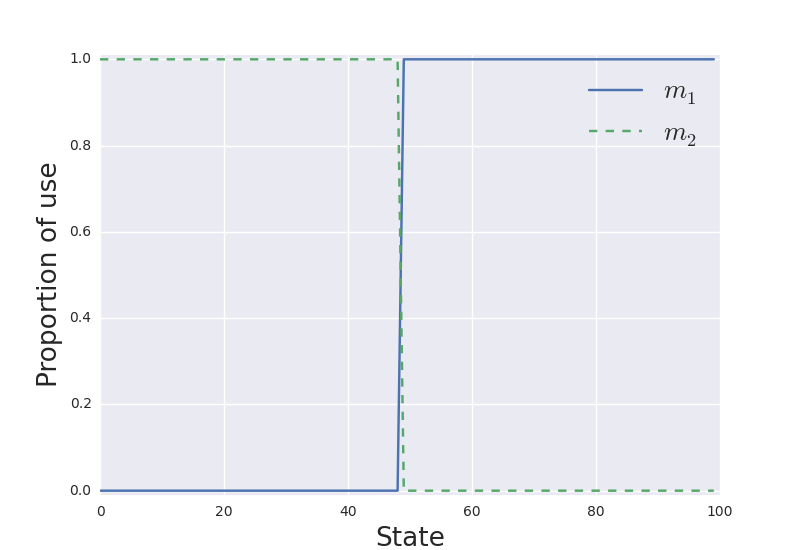
\includegraphics[scale=0.4]{../code/plots/vag-gen0.png}
    \caption{Initial ``crisp'' population}
  \end{subfigure}
  ~
   \begin{subfigure}[b]{0.45\textwidth}
    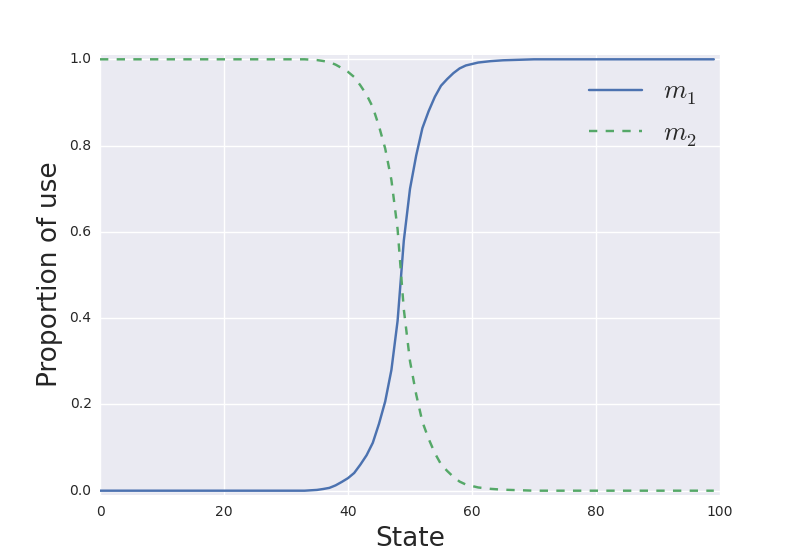
\includegraphics[scale=0.4]{../code/plots/vag-gen1.png}
    \caption{Second ``vague'' generation}
  \end{subfigure}
  \caption{Noisy iterated learning with $\sigma = 0.4$, $k = 20$ and $100$ sampled production sequences per parent (posterior sampling)}
  \label{fig:vag}
\end{figure}
 
\paragraph{Setup.}
\begin{itemize}
  \item $S = [0,99]$
  \item $|M| = 2$
  \item There is one signaling behavior per threshold $\theta$ and one threshold per state, i.e., $100$ types.
  \item $P(m_1|s,t) = 1$ iff $s \geq \theta_t$, otherwise $P(m_2|s,t) = 1$.
  \item $P(s_{\text{perceived}} | s_{\text{actual}})$ is the probability density of getting $s_{\text{perceived}}$ from $\text{Normal}(s_{\text{actual}},\sigma)$
  \item Data generated by teachers is sampled without noise to get a representative sample. But actual likelihoods of producing the data used to compute $Q$ are subjected to noise as above (as specified above)
  \item Learners are not aware of noise (as specified above)
  \item No replication.
\end{itemize}




\subsection{Deflation}
\paragraph{Main result.} Asymmetric and noisy perception can capture meaning deflation. See Figure \ref{fig:defl}.

\begin{figure}[ht]
\centering
    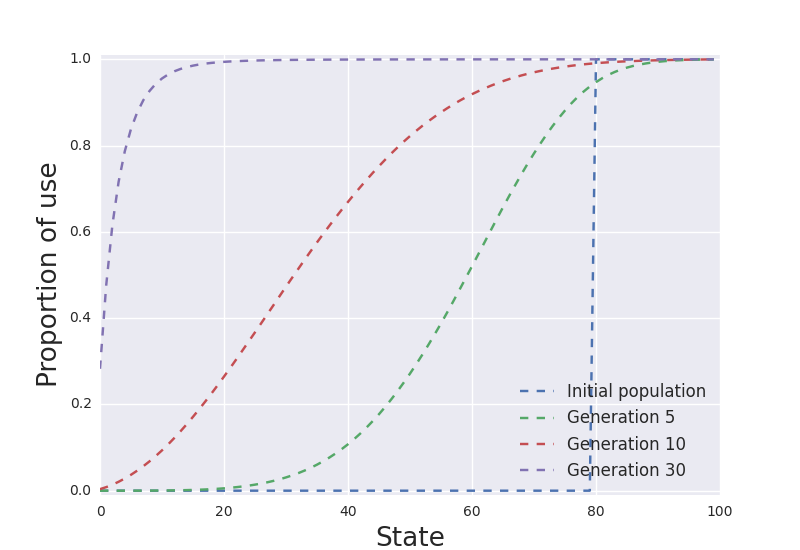
\includegraphics[scale=0.5]{../code/plots/deflation-sigma04.png}
  \caption{Noisy iterated learning with $\sigma = 0.4$, $k = 30$ and $300$ sampled production sequences per parent (posterior sampling)}
  \label{fig:defl}
\end{figure}

\begin{itemize}
  \item $S = [0,99]$
  \item $|M| = 1$
  \item There is one type of signaling behavior per threshold $\theta$ and one threshold per state, i.e. $100$ types.
  \item $P(m|s,t) = 1$ iff $s \geq \theta_t$, otherwise no message is sent. \tb{I'm pretty confident that adding some error-rate to this behavior wouldn't change the predictions. I left it deterministic for the time being}
  \item $P(s_{\text{perceived}} | s_{\text{actual}})$ is the probability density of getting $s_{\text{perceived}}$ from $\text{Normal}(s_{\text{actual}},\sigma)$
  \item $P(\theta | d) \propto (\prod_{s \in d} P(m|s,\theta)) \times \text{Binom}(\text{successes} = k-|d|, \text{trials} = k, \text{succ.prob} = \sum_{s'=0}^{\theta-1} P(s'))$, where the latter is the probability of a type not reporting $k-|d|$ events for a total of $k$ events.
  \item Data generated by teachers is sampled without noise to get a representative sample. But actual likelihoods of producing the data used to compute $Q$ are subjected to noise as above (as specified above)
  \item Learners are not aware of noise (as specified above)
  \item No replication. \tb{Not sure how this would work anyway. The higher $\theta$, the less a type communicates. If that's a communicative failure, then these types are even more dispreferred than with only learning. If it's not, then we have the same fitness for each type}
\end{itemize}

\subsection{Quantifiers}
\paragraph{Main result.} Noisy perception of states can mimic cognitive biases. In this case, a bias towards simplicity (no upper-bounds) as analyzed in \citet{brochhagen+etal:2016:CogSci}. Pragmatic inferences stabilize in population as byproduct of noise, as shown in Figure \ref{fig:quant}. Little changes for small increases of $k$ (10 or 15) or $l$ (e.g. 10 instead of posterior sampling).


\begin{figure}[ht]
\centering
    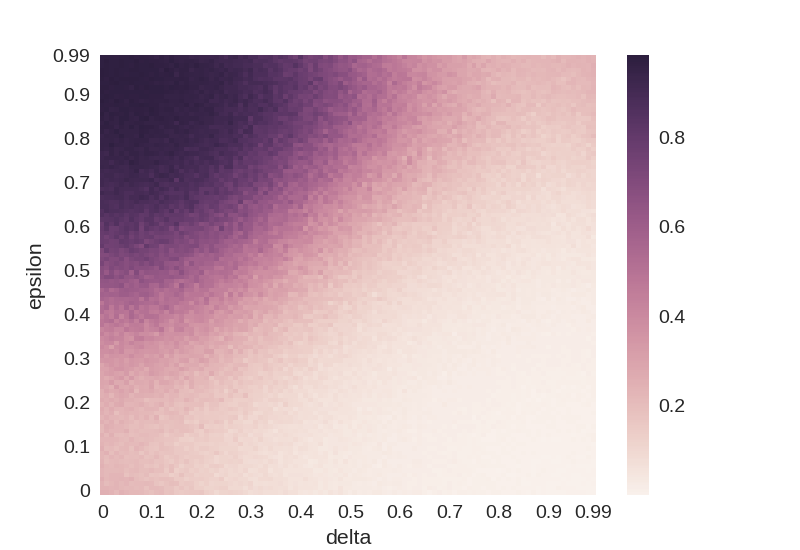
\includegraphics[scale=0.5]{../code/plots/quantifiers-posterior-sampling-k5.png}
  \caption{Influence of noise-parameters on the mean proportion of Gricean players with a lexicon lacking an upper-bound after $20$ generations with $k = 5, \lambda = 20, \alpha = 1$ and $10$ sampled production sequences per parent (posterior sampling).}
  \label{fig:quant}
\end{figure}
%

\begin{itemize}
  \item $S = \{\ssome, \sall\}$
  \item $|M| = 2$
  \item There are two lexica, one upper-bounded and one lacking upper-bound, and two signaling behaviors, literal and gricean, for a total of four lexica
  \item $P(m|s,t)$ is soft-maximizing literal or gricean behavior with $\alpha$ as exponent, using a type's lexicon -- as in our other setup \tb{Alternatively, we could go for simple Boolean behavior to keep everything uniform}
  \item $P(\ssome|\sall) = \delta$, $P(\sall|\ssome) = \epsilon)$
  \item Learners are not aware of noise (as specified above)
  \item No replication
\end{itemize}



\section{Discussion}
\tb{To be specified. Parts can be taken from our previous draft} 

\section{Conclusion}


\section{Acknowledgments}



\bibliographystyle{apacite}

\setlength{\bibleftmargin}{.125in}
\setlength{\bibindent}{-\bibleftmargin}

\bibliography{noise-bib}


\end{document}
